\documentclass{beamer}
\usetheme{ConnectivityLab}
\usepackage{times}
\usepackage{graphicx}
\usepackage{verbatim}
\usepackage{outlines}
\usepackage{fancyhdr}
\usepackage{subfigure}
\usepackage{cancel}
\usepackage{bibentry}
\usepackage{varwidth}
\usepackage{etoolbox}
\usepackage{epstopdf}

%%%%%%%%%%%%%%%%%%%%%%%%%%%%%%%%%%%%%%%%%%%%%%%%%%%%%%
%%%%%%%%%%%%%%%%%%%%%%%%%%%%%%%%%%%%%%%%%%%%%%%%%%%%%%

\title {
    Your Topic
}
\author {
    Speaker: Your Name
}
\date {
    January 13, 2016 %\today
}

%%%%%%%%%%%%%%%%%%%%%%%%%%%%%%%%%%%%%%%%%%%%%%%%%%%%%%
%%%%%%%%%%%%%%%%%%%%%%%%%%%%%%%%%%%%%%%%%%%%%%%%%%%%%%

\begin{document}
\begin{frame}
    \titlepage
\end{frame}

%%%%%%%%%%%%%%%%%%%%%%%%%%%%%%%%%%%%%%%%%%%%%%%%%%%%%%
%%%%%%%%%%%%%%%%%%%%%%%%%%%%%%%%%%%%%%%%%%%%%%%%%%%%%%

\begin{frame}{Outline}
    \tableofcontentsgather
    \tableofcontents
\end{frame}

%%%%%%%%%%%%%%%%%%%%%%%%%%%%%%%%%%%%%%%%%%%%%%%%%%%%%%
%%%%%%%%%%%%%%%%%%%%%%%%%%%%%%%%%%%%%%%%%%%%%%%%%%%%%%
\section{Introduction}

%%%%%%%%%%%%%%%%%%%%%%%%%%%%%%%%%%%%%%%%%%%%%%%%%%%%%%
%%%%%%%%%%%%%%%%%%%%%%%%%%%%%%%%%%%%%%%%%%%%%%%%%%%%%%
\begin{frame}{\textcolor{gray}{Use 2 lines -} \\ There is the 2 line Introduction test (1/2)}
    \begin{itemize}
        \item \textbf{First Layer 1}
        \begin{itemize}
            \item[-] Second Layer 1
            \begin{itemize}
                \item[+] Third Layer 1
                \item[+] $\Gamma(1+t)=t\Gamma(t)$
            \end{itemize}
        \end{itemize}

        \item \textbf{First Layer 2} \cite{Li15}
        \begin{itemize}
            \item[-] Second Layer 2 \cite{CPY11}
            \begin{itemize}
                \item[+] Third Layer 1 \cite{Meyn07}
                \item[+] Third Layer 2 \cite{Hartl1995}
            \end{itemize}
        \end{itemize}
    \end{itemize}
\end{frame}

%%%%%%%%%%%%%%%%%%%%%%%%%%%%%%%%%%%%%%%%%%%%%%%%%%%%%%
%%%%%%%%%%%%%%%%%%%%%%%%%%%%%%%%%%%%%%%%%%%%%%%%%%%%%%
\begin{frame}{Introduction (2/2)}
    \begin{figure}[t]
        \centering
        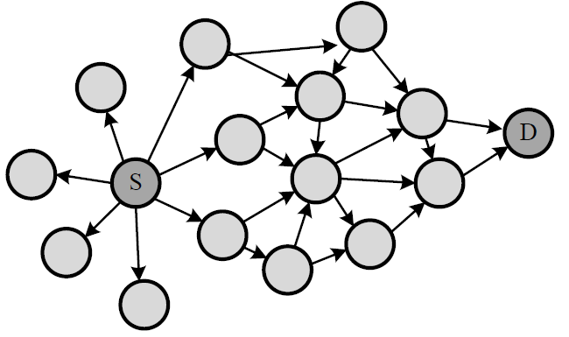
\includegraphics[width=0.6\textwidth]{figures/Fig_1-1.png}
        \setbeamerfont{caption}{size=\tiny}
        \caption{Some Figure Description}
    \end{figure}
\end{frame}

%%%%%%%%%%%%%%%%%%%%%%%%%%%%%%%%%%%%%%%%%%%%%%%%%%%%%%
%%%%%%%%%%%%%%%%%%%%%%%%%%%%%%%%%%%%%%%%%%%%%%%%%%%%%%
\section{Simulation}

%%%%%%%%%%%%%%%%%%%%%%%%%%%%%%%%%%%%%%%%%%%%%%%%%%%%%%
%%%%%%%%%%%%%%%%%%%%%%%%%%%%%%%%%%%%%%%%%%%%%%%%%%%%%%
\begin{frame}{Table}
    \begin{center}
        \begin{tabular}{ | l | l | }
            \hline
                Parameter                                   &       Value               \\ \hline
                Simulation Count                            &       100 thousand        \\ \hline
                Area Width / Length                         &       40.0 meter          \\ \hline
                eNB Intensity ($\lambda_{B}$)               &       0.01 $m^{-2}$       \\ \hline
                CeUE Intensity ($\lambda_{C}$)              &       0.15 $m^{-2}$       \\ \hline
                DeUE Intensity ($\lambda_{D}$)              &       0.15 $m^{-2}$       \\ \hline
                Path Loss Exponent ($\alpha$)               &       4.0                 \\ \hline
                eNB Power ($P_{B}$)                         &       43.0 dBm            \\ \hline
                Maximum Medium Access Prob. $\tilde{p}$     &       0.9                 \\
            \hline
        \end{tabular}
    \end{center}
\end{frame}

%%%%%%%%%%%%%%%%%%%%%%%%%%%%%%%%%%%%%%%%%%%%%%%%%%%%%%
%%%%%%%%%%%%%%%%%%%%%%%%%%%%%%%%%%%%%%%%%%%%%%%%%%%%%%
\begin{frame}{Table 2}
    \begin{columns}
        \column{0.15\textwidth}
        \column{0.3\textwidth}
        \fontsize{12pt}{16}\selectfont
        \begin{table}[h]
            \begin{tabular}{ | l | l | }
                \hline
                    \textbf{$N$}                                &       $100$             \\ \hline
                    \textbf{$\omega$}                           &       $1.3683$          \\ \hline
                    \textbf{$v_{min}$}                          &       $4$               \\ \hline
                    \textbf{$v_{max}$}                          &       $10$              \\ \hline
                    \textbf{$E[V^*_{RWP}]$}                     &       $8.7$             \\ \hline
                    \textbf{$E[V^*_{RD}]$}                      &       $7.4$             \\ \hline
                    \textbf{$L$}                                &       $4$               \\ \hline
            \end{tabular}
        \end{table}

        \column{0.6\textwidth}
        \begin{table}[h]
            \begin{tabular}{ | l | l | l | }
                \hline
                    \textbf{$\lambda_{RWP}$}                    &       $0.37043$          &            $0.14817$ \\ \hline
                    \textbf{$r$}                                &       $0.2489$           &            $0.0996$  \\ \hline
            \end{tabular}
        \end{table}

    \end{columns}
\end{frame}

%%%%%%%%%%%%%%%%%%%%%%%%%%%%%%%%%%%%%%%%%%%%%%%%%%%%%%
%%%%%%%%%%%%%%%%%%%%%%%%%%%%%%%%%%%%%%%%%%%%%%%%%%%%%%
\section{References}
\calcreferencespagetotal % Calc your References Page total number
\begin{frame}[allowframebreaks]{References}
    \fontsize{9pt}{13}\selectfont
    \bibliographystyle{IEEEtran}
    \bibliography{IEEEabrv,Citation}
\end{frame}

%%%%%%%%%%%%%%%%%%%%%%%%%%%%%%%%%%%%%%%%%%%%%%%%%%%%%%
%%%%%%%%%%%%%%%%%%%%%%%%%%%%%%%%%%%%%%%%%%%%%%%%%%%%%%
\section{}

\begin{frame}
    \centering
    \Large{Thanks for Your Attentions}
\end{frame}

\end{document}
